\NextFile{install.html}

\chapter{Installing Sailfish} \label{chap:install}
\index{Installing}
\index{Firmware!Installing}

This details the installation of Sailfish on a printer currently running \gls{firmware} other than Sailfish.  If your printer already has Sailfish installed, instead refer to Chapter~\ref{chap:update}.

It is important to note that if your printer is new to you, then you are advised to consider using it for at least a week before switching firmware.  This allows you to get to know your printer and ensure that it is operating correctly before upgrading it in any way.  If you upgrade a new printer before establishing that it is functioning properly, it may be difficult to distinguish between manufacturing defects and changes introduced by the modifications you have created.  Do yourself a favor and take things \textsl{s\,l\,o\,w\,l\,y}.

If you are unsure what firmware your printer is running, these steps can help you ascertain the firmware type.\index{Identifying firmware}\index{Firmware!Identifying}

\begin{enumerate}
\item If your printer does not have an LCD display, you will need to connect
  directly to it over USB and find what firmware version it reports.
  If it reports a firmware version of 3.1 or earlier, then it is running MakerBot's 
  stock firmware.  A firmware version of 3.2 or later means that it is running 
  either the Jetty Firmware, 3.2--3.5, or Sailfish, 4.0 and later.  (The Jetty Firmware is Sailfish
  by an earlier name.)  If the latter is the case, see Chapter~\ref{chap:update} for information
  on upgrading your printer's firmware.
\item If your printer does have an LCD display, then turn it on.  As it powers
  up, watch the LCD display for a ``splash'' screen which will appear only
  for a few seconds.  If Sailfish is running on your printer, then the splash
  screen should be similar to that shown in Figure~\ref{fig:splash}.  Look
  to see if the word ``Sailfish'' appears.  If it does, then your printer is
  already running Sailfish and you should turn to Chapter~\ref{chap:update}.
  Even if the word ``Sailfish'' does not appear, it is still possible that you
  are already running Sailfish, as some manufacturers alter the splash screen to
  show different information.
\item If you missed seeing the splash screen or are still unsure what firmware 
  you are running, check and see how many top-level menu items your printer 
  has.  Sailfish only has the three presented in Section~\ref{sec:Main}. 
  However, this is not definitive as early versions 
  of MakerBot's firmware display only three top-level menu items as well.  
  But, if you see more than three top level menu selections, as well as the printer 
  name which appears on the first line, then you are unlikely to be running Sailfish.
\item Finally, go to the ``Version Information'' item of the
  ``Utilities'' menu and see what is displayed.  Refer to
  Section~\ref{sec:versinf} for samples of the Sailfish version
  information screen.  If you do not see the word ``Sailfish'' in the
  display, then you are not running Sailfish.
\end{enumerate}

Once you are satisfied that your printer is \emph{not} running Sailfish
\emph{and} you are ready to upgrade to Sailfish, then read on.  But please
follow these directions carefully so as to prevent any surprises that may delay
your return to printing.

\begin{bclogo}[logo=\bcinfo, noborder=true, couleurBarre=yellow]{Note}
On Replicator series printers, the Sailfish version numbers begin at 6.2.
On Thing-o-Matic and Cupcake printers, Sailfish version numbers begin at 4.0.
\end{bclogo}

\NextFile{install-hardware-reqs.html}

\section{Hardware Requirements}
\index{Requirements!Hardware}

Sailfish runs on \gls{MightyBoard} rev~E, G \& H as well as \gls{Gen 3} and
\gls{Gen 4} electronics.\index{MightyBoard}\index{Gen 3}\index{Gen 4}
For all Replicators, both single and dual extrusion is supported.  Specific per
machine requirements are as detailed below.  Note that each printer category
also supports the clones of the printers listed in that category.  For instance, The
Replicator 1 includes CTC, FlashForge, MBot3D, WanHao, ZYYX, and
other Replicator 1 ``clone'' printers.

\begin{enumerate}
\item \strong{The Replicator 2 and 2X:} MakerBot MightyBoard rev~G or H
electronics with one or two extruders.
\item \strong{The Replicator 1:} MakerBot MightyBoard rev~E electronics with
  one or two extruders.
\item \strong{Thing-o-Matics:} MakerBot v2.X motherboard, MakerBot v3.6
Extruder Controller, MakerBot v3.3 Step\-per Dri\-vers, a stepper-based extruder,
and an Arduino Mega or Arduino Mega 2560. Other than the extruder, these are
all ``stock'' Thing-o-Matic electronics; i.e., Gen 4 electronics. Stepper-based
extruders include the Mk6, Mk6+, Mk7, and Mk8.  Other electronics and extruders
may or may not work with the Sailfish firmware.
\item \strong{Cupcakes with Gen 4 electronics:} As per the requirements for
  Thing-o-Matics.
\item \strong{Cupcakes with Gen 3 electronics:} Stepper motor extruder plus
 the 3G5D Shield or the ``Ugly Cable Hack'' to control the stepper motor
 extruder.  Additionally, the remaining complement of Gen 3 electronics: RepRap
 Motherboard v1.2, Plastruder Extruder Controller, and v2.3 or later stepper
 drivers.\index{3G5D shield}\index{Ugly cable hack}
\end{enumerate}

If your printer does not satisfy the above requirements, then Sailfish
likely will not run on it.  For example, Sailfish does not presently
support RAMBo, RAMPS, or other common RepRap electronics.

\NextFile{install-hardware-reqs-cupcakes-and-thingomatics.html}

\subsection{Cupcakes and Thing-o-Matics}

If you are using a Cupcake or Thing-o-Matic, you must know the type of
motherboard that you have.  For Gen~4 electronics, this will be an Arduino Mega
or Arduino Mega 2560 and will appear in ReplicatorG's Firmware Upgrade
window as ``MakerBot Thing-o-Matic (Gen 4)'' or ``MakerBot Thing-o-Matic
(Gen 4) with ATmega 2560''.  For Gen~3 electronics --- Cupcakes --- this will
be a RepRap Motherboard v1.X and will appear in ReplicatorG as
``MakerBot Cupcake 3G 5D Shield (Gen 3)''.

If you don't know the Cupcake or Thing-o-Matic board type, stop now
and inspect your printer to determine the type of board you have
installed.  For Thing-o-Matics, you will need to open up the printer's
bottom to inspect the board. You may even have to remove the ``motherboard''
from the Arduino board.  If that is the case, then carefully remove it,
lifting straight up.  When re-attaching it, be careful to not bend any
of the pins.

\NextFile{install-hardware-reqs-flashforge.html}

\subsection{FlashForge printers built after April 2014}

Some FlashForge printers manufactured after April 2014 come equipped with
an ATmega 2560 microprocessor, often simply referred to as a ``2560''.  Having
a 2560 is a nice upgrade: that processor has twice the program space of
the processor found in genuine MakerBots. It supports additional firmware
features.

If you have a FlashForge with a 2560, then you must be sure to use the
appropriate 2560 firmware; for instance, the firmware listed as ``FlashForge Creator
X with ATmega 2560''.  If you are unsure of which processor your FlashForge
has, turn it over, open the electronics bay, and look for the large, black
square chip.  Under good light and with a magnifying glass, read the printing
on it and see if it says ``1280'' or ``2560''.

\NextFile{install-software-reqs.html}

\section{Software Requirements} \label{sec:soft-reqs}
\index{Requirements!Software}

The Sailfish firmware may be installed on either \textit{bona fide} or
``clone'' versions of the Replicator 1, Replicator 2, Replicator 2X,
Thing-o-Matic, and Cupcake printers.  For some clone printers, special
versions of Sailfish are distributed to accomodate their mechanics (e.g.,
the spacing of dual extruders) or to leverage their special features
(e.g., bigger power supplies for faster heating, auto-leveling, etc.).

Sailfish requires the use of the ``ReplicatorG 40 -- Sailfish'' computer
software in order to install the Sailfish firmware.  As of this writing,
you cannot use either MakerBot MakerWare or Desktop to install Sailfish on
any printer except for Thing-o-Matics. Download ReplicatorG 40 -- Sailfish
from the \myhref{http://www.thingiverse.com/thing:3208}{Thingiverse ``Thing''
number 32084}.

\begin{bclogo}[logo=\bcattention, noborder=true, couleurBarre=red]{Important!}
You must use ReplicatorG~40 -- Sailfish.  Do not use the abandoned
ReplicatorG 0040 as it does not correctly handle ``onboard parameters'' in
MakerBot or Sailfish firmwares 7.0 or later.  You can tell that you are
running ReplicatorG~40 -- Sailfish as that exact name will appear in the
running application's window title bar, as seen in
Figure~\ref{fig:repg-version}.  You can also use the ``About'' item from the
application's menu.  Note that the version information also includes a
revision number; e.g., ``0040r27'' is version 40,
revision 27.\index{ReplicatorG!Version}
\end{bclogo}

\begin{figure}[!htbp]
  \centering
    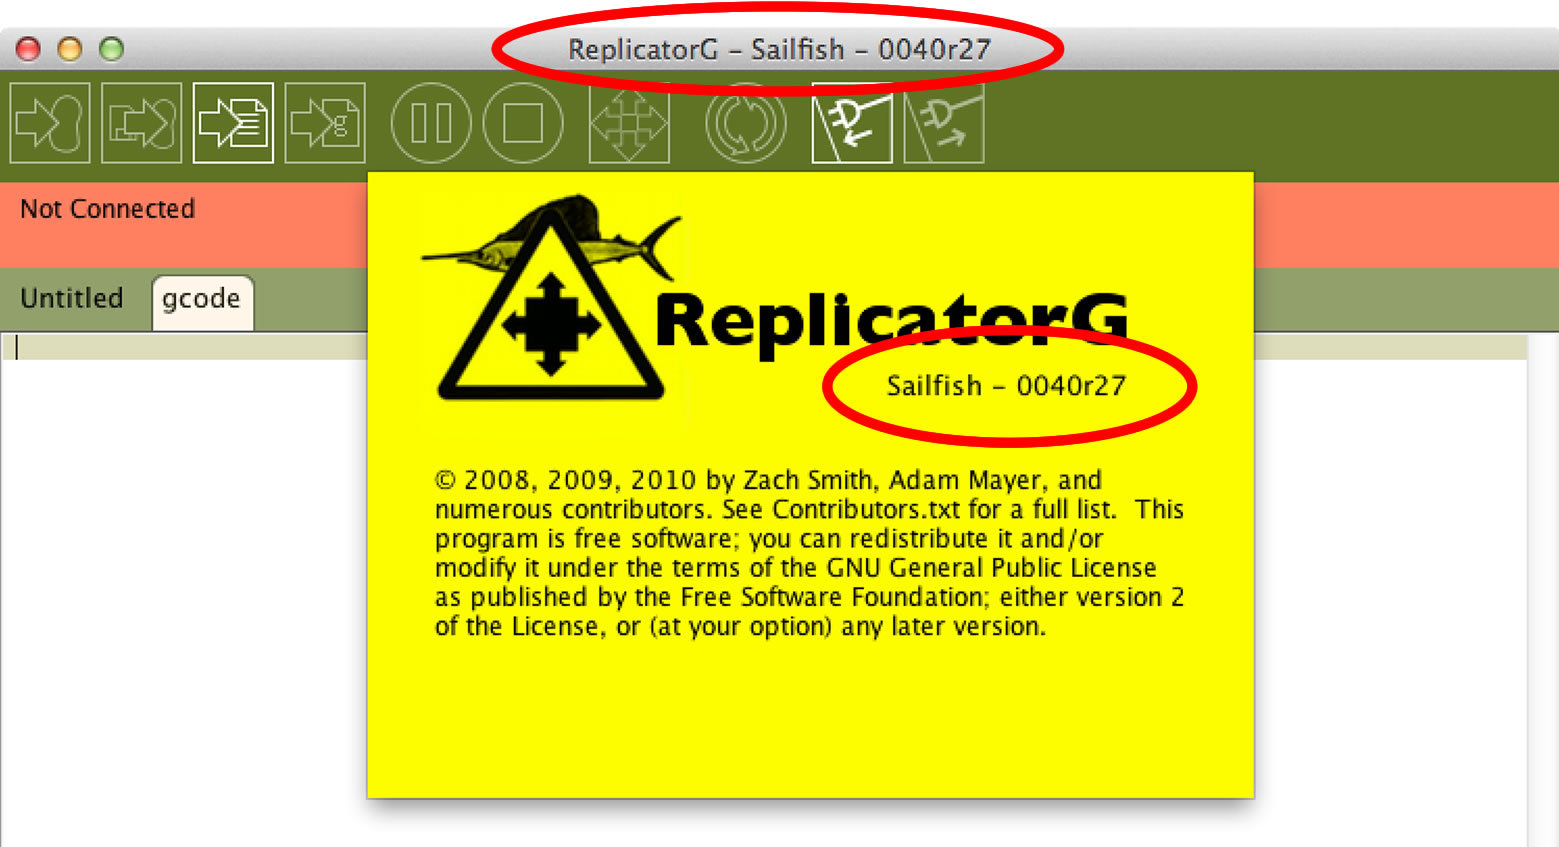
\includegraphics[width=5in]{repg-version}
    \caption{ReplicatorG: version information}
  \label{fig:repg-version}
\end{figure}

Thing-o-Matic and Cupcake operators should note that, as of Sailfish
4.4, use of \gls{Volumetric 5D gcode} is required.  \gls{RPM gcode} is
no longer supported.  If you still use Skeinforge, then you must use
Skeinforge-50.  Note that Cura, KISSlicer, MakerWare, Simplify3D,
Skeinforge 50, and slic3r all produce Volumetric 5D
gcode.\footnote{For Cura, KISSlicer, and slic3r you must convert the
  gcode to \gls{X3G}.  To this end, you may use GPX to convert gcode to X3G.
  GPX is available on github,
\myhref{https://github.com/whpthomas/GPX}{https://github.com/whpthomas/GPX}.  Use of X3G
  is not unique to Sailfish: it is required by the stock MakerBot
  firmware as well.\index{GPX}}

\NextFile{install-installing.html}

\section{Installing}
\index{Installing|(}

For the best installation outcome, please read once through all of these
steps before installing Sailfish.  Then, as you install Sailfish, carefully
reread and follow each step.

\NextFile{install-installing-step-1.html}

\subsection{Step 1: Before you install Sailfish} \label{sec:preinstall}

Before installing Sailfish, power on your printer, connect it to your computer
via USB, and then run MakerWare.  Using MakerWare, write down the following
machine onboard parameters:

\begin{enumerate}
\item The X, Y, and Z home offsets.  These are also referred to
  as ``home positions''.
\item If your printer has two extruders, write down the X and Y toolhead
  offsets.
\end{enumerate}

\begin{bclogo}[logo=\bcattention, noborder=true, couleurBarre=red]{Important!}
You must use MakerBot MakerWare or Desktop to obtain these values: ReplicatorG
will not correctly read them from ``stock'' MakerBot firmware of version 7.0
or later.  If you do not have MakerWare or Desktop, then download it from
makerbot.com.
\end{bclogo}

\NextFile{install-installing-step-2.html}

\subsection{Step 2: Stop MakerWare's background services} \label{sec:conveyor}

MakerWare, when installed, runs a background service known as ``Conveyor''.
After running MakerWare as per the prior section, you must stop Conveyor.
Otherwise, Conveyor will prevent ReplicatorG from downloading firmware to
your printer.  After you have installed Sailfish, you can restart Conveyor if
you wish.  However, do not do so until you have completely finished installing
and configuring Sailfish.

To stop Conveyor,\index{Conveyor, stopping}\index{MakerWare!Conveyor} first
launch MakerWare if it is not already running.  From MakerWare's ``Services''
menu, select the ``Stop Background Service'' item. To restart Conveyor later,
use the ``Restart Background Service'' item from that same menu.

\NextFile{install-installing-step-3.html}

\subsection{Step 3: Obtain ReplicatorG 40 -- Sailfish}
\index{ReplicatorG!Obtaining}

Next, if you have not already done so, download and unpack ReplicatorG~40 --
Sailfish from the
\myhref{http://www.thingiverse.com/thing:32084}{Thingiverse ``Thing''
number 32084}.

You do not need to use ReplicatorG as your \gls{slicer}: you may continue using
whatever \gls{slicer} you prefer.  You only need ReplicatorG to install or update
Sailfish.  On Windows systems, just unzip the ReplicatorG download and place
the folder on your desktop.  Then run the \texttt{replicatorg.exe} program
directly from that unzipped folder.

\NextFile{install-installing-step-4.html}

\subsection{Step 4: Obtain Sailfish} \label{sec:download-url}

Start ReplicatorG; then, from the ``Preferences'' item of the main menu,
click the ``Advanced'' button.  Verify that the ``Firm\-ware update
URL'' field reads,
\begin{quote}
{\hspace{-30pt}\smaller\texttt{http://jettyfirmware.yolasite.com/resources/release/firmware.xml}}
\end{quote}
as depicted in Figure~\ref{fig:download-url}. Then click ``Close''.

\begin{figure}[!htbp]
  \centering
    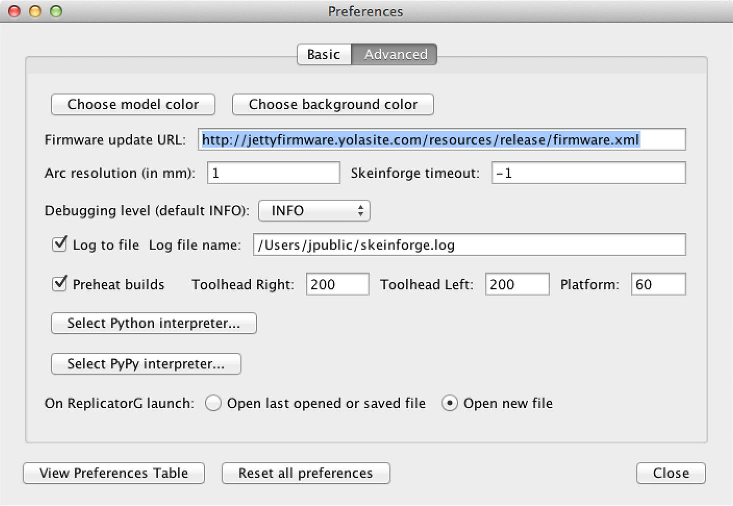
\includegraphics[width=5in]{download-url}
    \caption{Sailfish download location}
  \label{fig:download-url}
\end{figure}

After a brief pause, ReplicatorG should start logging the firmware files it
downloads; e.g., in the bottom portion of the ReplicatorG window you will
see messages similar to

{\smaller\tt\begin{verbatim}
34891 bytes written to firmware.xml
353301 bytes written to mighty_twox-Sailfish-v7.6.0-r1220.hex
353174 bytes written to mighty_twox-Sailfish-v7.6.0-r1220b.hex
354823 bytes written to mighty_twox-Sailfish-v7.5.0-r1135.hex
...
\end{verbatim}}

If you don't see such messages after a minute, exit and restart ReplicatorG.
You do need to be connected to the Internet in order for the download to
succeed.  Note that using a firewall proxy will probably not be successful.

\NextFile{install-installing-step-5.html}

\subsection{Step 5: Thing-o-Matics: update the extruder controller firmware}
\index{Thing-o-Matic!Extruder controller}

This section is only applicable to Thing-o-Matics.  For other printers,
skip to the next section.

The Sailfish firmware is a derivative of version 3.1 of the motherboard
firmware.  Consequently, you must first ensure that your Thing-o-Matic's
Extruder Controller (EC) is updated to v3.1 EC firmware. Thing-o-Matic owners
should complete this step before beginning the next step.  To obtain
EC firmware, point ReplicatorG's download URL to
\begin{quote}
{\smaller\texttt{http://firmware.makerbot.com/firmware.xml}}
\end{quote}
And then follow Makerbot's EC firmware upgrade procedures.  After you are
done, point the download URL back to the Sailfish site described in Section \ref{sec:download-url}.

\NextFile{install-installing-step-6.html}

\subsection{Step 6: And now, install Sailfish} \label{sec:really-install}
\index{Installing}
\index{Firmware!Types}

Connect your printer's USB cable to both the printer and the computer from
which you will be performing the upgrade.  Next, power your printer on --- but
do not connect from ReplicatorG to the printer. Check the ``Connection (Serial
Port)'' submenu of ReplicatorG's ``Machine'' menu.  Make sure that you see the
USB port for your printer listed. If it does not appear, then select the
``Rescan serial ports'' item of said sub-menu as seen in
Figure~\ref{fig:repg-rescan}. You cannot proceed
until your printer's serial port appears.

\begin{figure}[!htbp]
  \centering
    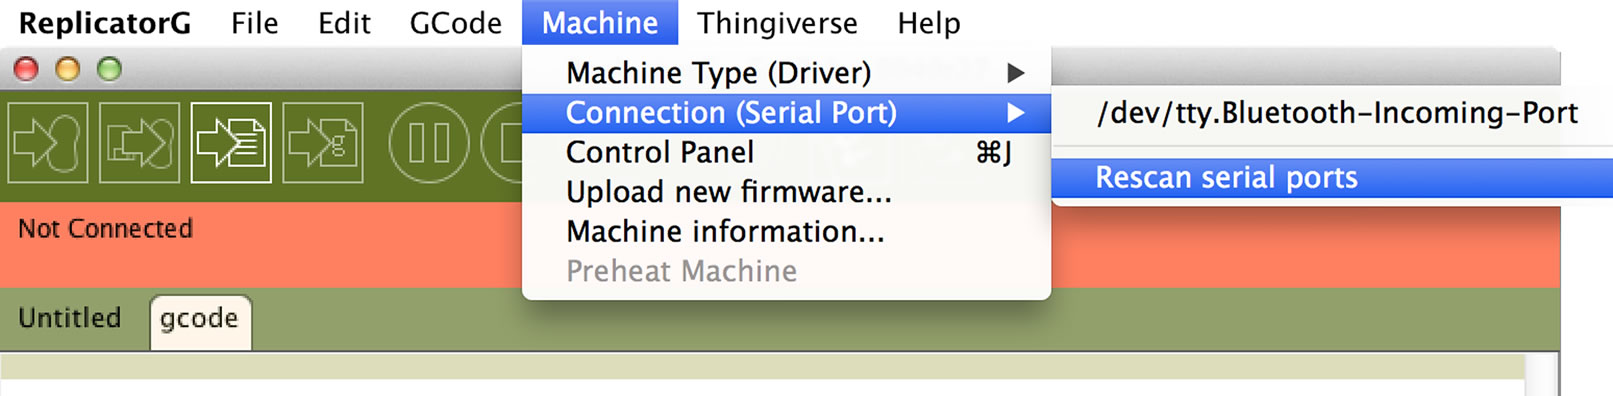
\includegraphics[width=5in]{repg-rescan}
    \caption{ReplicatorG: rescan serial ports}
  \label{fig:repg-rescan}
\end{figure}

Again, \emph{do not} actually connect from ReplicatorG to the printer: the
firmware upload process itself will perform that step itself and will
\emph{fail} if ReplicatorG is already connected.

From ReplicatorG select the ``Upload New Firmware'' submenu of the
``Machine'' menu. You will see different printers listed, including
those listed below.  Note that new printers are added when needed.  If
you do not see your printer type listed, then select the printer for
which it is a clone --- often the Replicator 1.

\begin{itemize}
\item MakerBot Replicator 2X
\item MakerBot Replicator 2X with ATmega 2560
\item MakerBot Replicator 2
\item MakerBot Replicator 2 with ATmega 2560
\item MakerBot Replicator 1 Single \& Dual
\item MakerBot Replicator 1 Single \& Dual with ATmega 2560
\item FlashForge Creator I, II \& X
\item FlashForge Creator X with ATmega 2560
\item Wanhao Duplicator 4
\item Core-XY MightyBoard revE
\item Core-XY MightyBoard revE with ATmega 2560
%\item ZYYX
\item MakerBot Thing-o-Matic (Gen 4)
\item MakerBot Thing-o-Matic (Gen 4) with ATmega 2560
\item MakerBot Cupcake 3G 5D Shield (Gen 3)
\end{itemize}

\noindent After selecting the printer type, click the ``Next'' button.

You should then see different firmware versions listed.  Unless you
have cause to do otherwise, select the most recent version --- the
highest numbered one.  Note that any versions
ending in the letter ``b'' are for printers with broken \gls{SD card} hardware.
Only select a ``b'' version if you know that you need to.  Also,
when you click on a given version, any specific requirements for
that version will be listed on the right hand side.  Typically this
includes the recommended revision of ReplicatorG.  Remember that you
can use any \gls{slicer} with Sailfish; this is just a recommendation of the revision
to use if you wish to use ReplicatorG to manipulate firmware parameters
stored on the printer via the ``Onboard Parameters'' screen of ReplicatorG.

Once you have selected the firmware version, click the ``Next'' button.
Then select the USB port to which your printer is connected.  Again, click the
``Next'' button.

Depending upon the type of printer you have, you will next be instructed
either to simply click ``Upload'', or to press your printer's mechanical reset button
while simultaneously clicking the ``Upload'' button on your computer screen.
For the Replicator 2 and 2X, there is no mechanical reset button and thus
no need to press one.  For most other printers, there may be one and you may
need to press it.  Refer to the documentation you received with the printer.
When having to press a reset button, the timing can be tricky and frustrating,
especially on Windows systems.  It sometimes works best to press the reset
button, then about a half second later, click the ``Upload'' button
on your screen.

Once the firmware has successfully downloaded, you are ready to
configure Sailfish!\index{Installing|)}
\ifpdf
\else
Proceed to the next section for instructions on configuring Sailfish for your printer.
\fi

\NextFile{install-configuring.html}

\section{Configuring}
\index{Configuration!Initial|(}

Now that you have installed Sailfish for the first time, there are some
first-time configuration steps you must take.  The non-Sailfish firmware
which was previously loaded may have stored different information in
the printer's non-volatile \gls{EEPROM} memory --- the memory which stores
configuration information and is saved even when the printer is turned off.
Having incorrect values stored will disrupt your printing.  Fortunately,
it is easy to reset the information to factory defaults.

Before following these steps, ensure that you use ReplicatorG 40 -- Sailfish.
You \emph{must not} use the abandoned ReplicatorG 0040 as it will not
correctly handle EEPROM settings for Sailfish or even stock 7.0 or later
firmware.  See Section~\ref{sec:soft-reqs} if you are unsure of which version
of ReplicatorG you have.

While it is possible to use MakerWare to set EEPROM parameters for
Sailfish as per Section~\ref{sec:makerware}, it is not convenient to
do so as some of the settings you must check are in units of
millimeters, whereas MakerWare will display them in units of stepper motor
steps.

\NextFile{install-configuring-step-7.html}

\subsection{Step 7: Establish factory defaults}

Now it is time to reset the printer's onboard settings to factory defaults.
This will ensure that all important settings are correct.  It will
also attempt to preserve any calibrations, cumulative print time
counters, and filament usage counters.

The simplest way to reset the printer to factory defaults is to
power on your printer and then, from the front panel display, select
the ``Utilities'' item in the main menu.\footnote{Refer to
Section~\ref{sec:Main} if you are not yet
familiar on how to navigate menus on the front panel.}  From the
``Utilities'' menu, select the ``Restore Settings'' item, which you will
find near the end of the list.  After selecting it, confirm the operation.
At that point, your printer will set itself to factory defaults and
then ``reboot'' itself.

Through ReplicatorG's ``Onboard Preferences'' screen, the printer may
also be reset to factory defaults.  Use that method if you prefer.

\NextFile{install-configuring-step-8.html}

\subsection{Step 8: Restore offsets} \label{sec:checkoffsets}

Next you need to check and, if need be, restore the offsets saved in
Step~1, Section~\ref{sec:preinstall}.  You may accomplish this
using either the printer's front panel or ReplicatorG.  Both methods
are described below.

You may also wish to check and set the extruder count and presence of
any heated build platform (\gls{HBP}).  The extruder count should be two if
you have two extruders and one otherwise.  Both of these checks may be
done from the printer's front panel.  See Sections~\ref{sec:extruder-count}
and \ref{sec:hbp-present}.

If you failed to do Step~1, then you can set the offsets to the
defaults for your printer as per Table~\ref{tab:default-offsets}.  If
you have two extruders, then you can set the X and Y toolhead offsets
each to 0~mm and, when you are ready to do \gls{dualstrusion} prints,
calibrate your toolhead offsets as per the directions in
Section~\ref{sec:toolheadoffsets}.
Note that Thing-o-Matics and Cupcakes do not have default values for their
home offsets: they are determined by running their calibration scripts.

\NextFile{install-configuring-step-8-ui.html}

\subsubsection{With the front panel}

You may inspect and change the home offsets using the ``Home Offsets'' item of
the ``Utilities'' menu.  See Section~\ref{sec:homeoff}
for directions on using that menu.  If your
printer has two extruders, then you must also check and, if necesssary,
restore, the toolhead offsets.  With Sailfish~7.7 or later, this may be done
with the ``Toolhead Offsets'' item of the ``Utilities'' menu as per
Section~\ref{sec:tooloff}.  If you have
Sailfish~7.6 or earlier, then you must use ReplicatorG to perform this
important step.

\NextFile{install-configuring-step-8-repg.html}

\subsubsection{With ReplicatorG 40 -- Sailfish} \label{sec:machine-type}
\index{ReplicatorG!Driver}
\index{ReplicatorG!Machine type}

Before connecting ReplicatorG to your printer, you must tell ReplicatorG the
correct machine type for your printer.  Otherwise, ReplicatorG may send
incorrect configuration information to your printer.

With your printer's USB cable \emph{not} connected to your computer, start
ReplicatorG.  It is important that the printer not be connected; otherwise,
ReplicatorG may automatically connect to your printer using the wrong
machine type.\footnote{ReplicatorG has a preference option to automatically
connect on startup. It is okay to use that feature \emph{after} you have completed
configuration of Sailfish.}

Next, with ReplicatorG's ``Machine'' menu, select a ``Machine Type (driver)''
matching your machine \emph{and including} ``(Sailfish)'' in the name; e.g.,
in Figure~\ref{fig:repg-driver} a dual extruder Replicator~1 is selected.

\begin{figure}[!htbp]
  \centering
    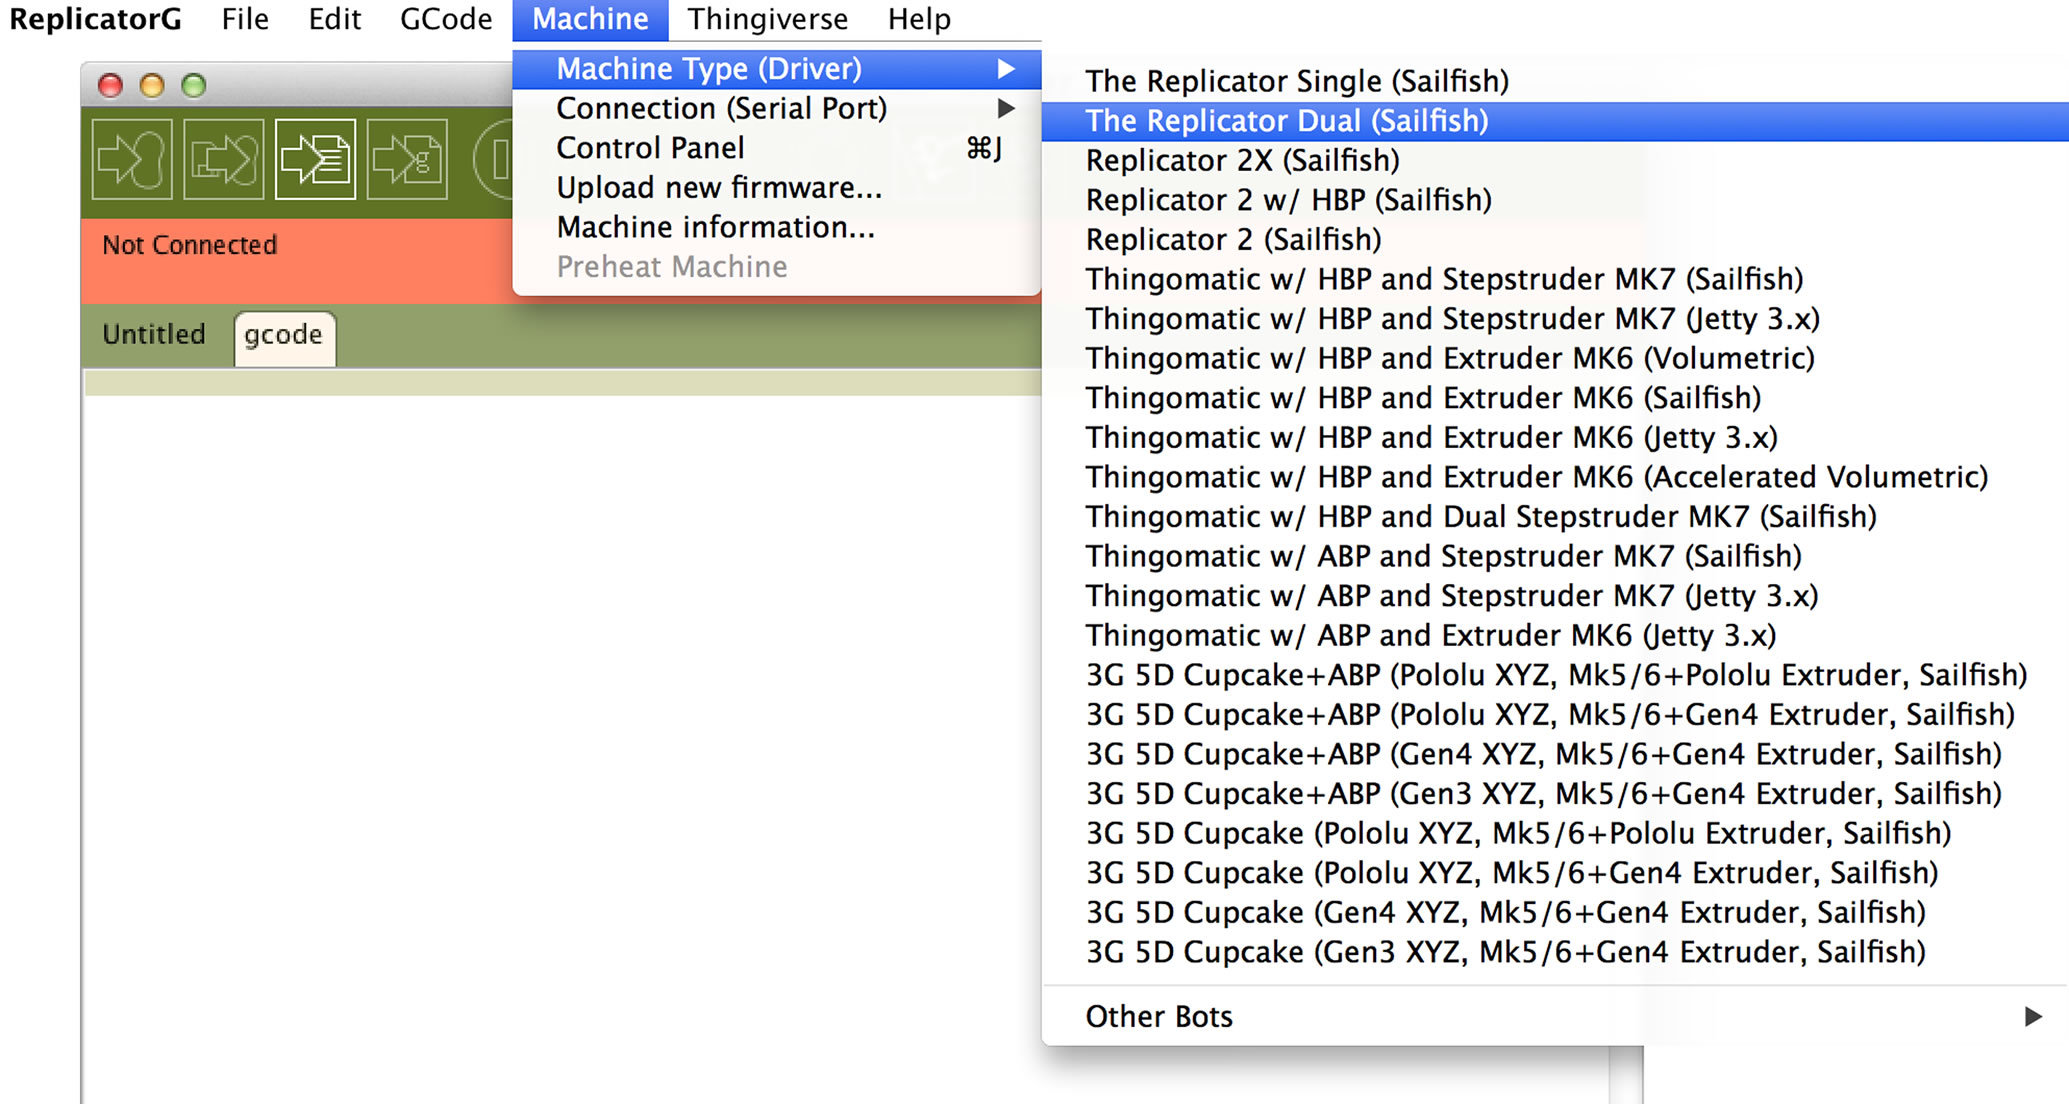
\includegraphics[width=5in]{repg-driver}
    \caption{ReplicatorG: selecting the machine type}
  \label{fig:repg-driver}
\end{figure}

If your printer is a Replicator~1 clone, then use one of the Replicator~1 types:
you will not see brand specific types such as WanHao Duplicator~4 or
FlashForge Creator~X.  Those brands are typically all Replicator~1 clones.

If you do not see machine types such as those shown in
Figure~\ref{fig:repg-driver}, then check to make sure that you are indeed
running ReplicatorG 40 -- Sailfish.  Other versions of ReplicatorG may not
include those machine types.

After selecting the machine type, connect your printer to your
computer via the USB cable and power it on. In ReplicatorG's ``Machine'' menu,
select the ``Rescan serial ports'' item under ``Connection (Serial Port)'' as
seen in Figure~\ref{fig:repg-rescan}.
Then, select the appropriate serial port under that same menu.  If you do
not see your printer's serial port then you will need to investigate why
it does not appear.  Diagnosing that issue is outside the scope of this
document.\footnote{The USB support in your printer is part of a separate
microprocessor.  It is not part of the Sailfish firmware.}

With the proper serial port selected, click ReplicatorG's ``connect'' icon
as shown in Figure~\ref{fig:repg-connect}.

\begin{figure}[!htbp]
  \centering
    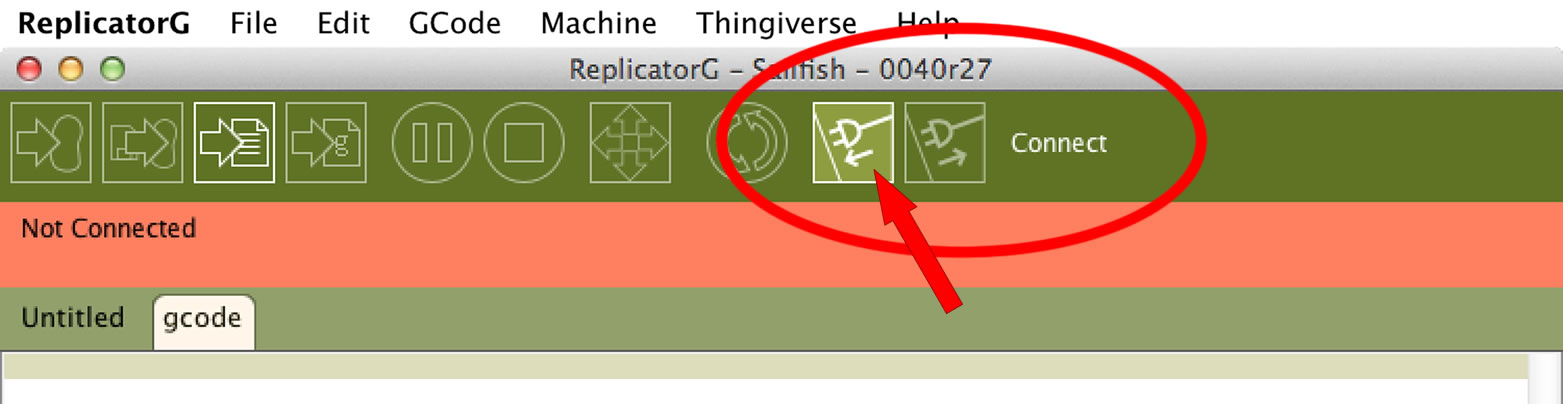
\includegraphics[width=5in]{repg-connect}
    \caption{ReplicatorG: connect to your printer}
  \label{fig:repg-connect}
\end{figure}

After a few seconds, ReplicatorG should indicate that you are now connected
to your printer.  If connecting fails, then there may be a USB communications
issue with your printer.  If you see a message about an incorrect ``toolhead
count'', do not worry.  This just indicates that you need to set the number
of extruders.  You can do that via ReplicatorG or using the printer's
``Utilities'' menu as per Section~\ref{sec:extruder-count}.

Under ReplicatorG's ``Machine'' menu select the ``Onboard Preferences''
item.  In the resulting window, select the ``Homing/VREF'' tab (simply
``Homing'' for Cupcakes and Thing-o-Matics).  Under that tab, check that
the X, Y, and Z home offsets are as you noted in Step~1.  Likewise, check
the X and Y toolhead offsets if you have two extruders.  Change any values
which are not correct and then press the ``Commit'' button.  Note that the
exact values you entered may not be precisely what is saved: the printer
converts the values to units of stepper motor steps.  When converted back
again to units of millimeters for display in ReplicatorG, the values will be
slightly different.  This is normal.
\index{Configuration!Initial|)}

\NextFile{install-makerware.html}

\section{MakerBot MakerWare \& Desktop and onboard parameters} \label{sec:makerware}

\index{MakerWare!EEPROM maps}
As mentioned previously, all the common \glspl{slicer} may be used with
Sailfish, including MakerBot MakerWare and MakerBot Desktop.  Moreover,
MakerBot Desktop comes with the necessary ``EEPROM maps'' to set ``onboard
parameters'' in Sailfish.  This means that you do not need to use ReplicatorG
for checking or changing onboard parameters: you may use Desktop.  However,
MakerWare 2.4 lacks these maps.  But you can install them yourself by
downloading them from the
\myhref{http://www.thingiverse.com/thing:32084}{Sailfish ``Thing''}
at thingiverse.com.  Look for the MakerWare EEPROM maps in the download list.
It is a ``zip'' file which you may download, unpack, and then install as per
the directions in the \texttt{README.txt} file included in the package.

\NextFile{install-removing.html}

\section{Removing Sailfish}
\index{Firmware!Removing}

Should you wish to remove Sailfish from your printer, you may do so at
any time.  This is accomplished by installing a different firmware as
per that firmware's installation and setup procedures.  For example,
to install ``stock'' MakerBot firmware (which may or may not be
appropriate to a clone printer), run MakerWare and allow it
to install official MakerBot firmware.  Alternatively, you can change
ReplicatorG's firmware download URL in the ``Advanced'' section of
the ``Preferences'' menu to,
\begin{quote}
{\smaller\texttt{http://firmware.makerbot.com/firmware.xml}}
\end{quote}
When installing a different firmware, it is generally a good idea to use
that firmware's method of resetting the printer to ``factory defaults''.  How
that is accomplished will depend upon the firmware with which you replace Sailfish.
